\documentclass[12pt,a4paper, oneside]{article}
\usepackage[utf8]{inputenc}
\usepackage[T1]{fontenc}
\usepackage[english,german]{babel}
\usepackage[style=german]{csquotes}
\usepackage{graphicx}

\author{Uni Oldenburg, SWP2020 Gruppe A}

\begin{document}
\begin{titlepage}									
\pagestyle{empty}									
\begin{center}

\begin{figure}[h]									
\centering											

\includegraphics[width=0.35\textwidth]{../img/Logo.jpg}
\end{figure}		

\bigskip \bigskip \noindent							
\textsc{\textbf{\LARGE Softwareprojekt:}} \par \bigskip \noindent																			
\textsc{\textbf{\LARGE Projekttagebuch}} 			    
													
													
\par \bigskip \bigskip \bigskip \bigskip \bigskip \noindent
{\Large Gruppe A} \par \medskip \noindent
		
\par \bigskip \bigskip \bigskip \bigskip \bigskip \bigskip \noindent																		
\textit{\Large Wintersemester 2020/21 und} \par \noindent
\textit{\Large Sommersemester 2021}				
													
\par \bigskip \bigskip \bigskip \bigskip \bigskip \bigskip \noindent			
\par \bigskip \bigskip \bigskip \noindent
{\Large Sprintanalyse} \par \medskip \noindent
		
\end{center}
\end{titlepage}

\tableofcontents
\pagebreak

\section{Sprinttagebuch: Sprint-Nr. 6}
\underline{Name des Sprints:}
\\
Sprint 6: Tohuwabohu Total

\noindent
\\
\underline{Zeitraum des Sprints:} 
\\
18. Februar 2021 - 09. März 2021

\noindent 
\\
\underline{Ziel des Sprints:} 
\\
Große Teile der Spiellogik, Verbesserung der User Experience, Entwicklertools, diverse Bugfixes und Dokupflege

\noindent
\\
\underline {Team:} 
\\
Sven Ahrens, Alwin Bossert, Aldin Dervisi, Marvin Drees, Mario Fokken,
Timo Gerken, Finn Haase, Temmo Junkhoff, Maximilian Lindner, Steven Luong, Phillip-André Suhr, Eric Vuong


\section{Vorgänge}

\begin{itemize}

\item SWP2020A-115: SecurityException bei nicht eingeloggten Clients bei Lobbyerstellung (3 Story Points)

\item SWP2020A-122: Fenster sollen Mindestdimensionierung bekommen (1 Story Point)

\item SWP2020A-124: ANmi bei der Registrierung meine Emailadresse angeben können (2 Story Points)

\item SWP2020A-128: ANmi, dass ich am Anfang meine Zuges würfeln kann (7 Story Points)

\item SWP2020A-129: ANmi, dass ich mit anderen Nutzern Ressourcen tauschen kann (13 Story Points)

\item SWP2020A-133: ANmi bei der Bank Entwicklungskarten kaufen können (12 Story Points)

\item SWP2020A-134: ANmi in meinem Zug eine Entwicklungskarte spielen können (8 Story Points)

\item SWP2020A-148: ChatMessageDTO nutzt UTC als Zeitzone, sollte Client-Zeitzone nutzen (2 Story Points)

\item SWP2020A-151: ANmi, dass beim Einloggen über einen neuen Client der ältere mit einer Warnung ausgeloggt wird, damit ich immer nur in einem Client angemeldet bin (3 Story Points)

\item SWP2020A-152: AEmi Zugriff auf ein Fenster haben, in dem ich manuell Requests, Messages, etc. auf den Bus legen kann, damit ich diese möglichst direkt ausprobieren kann (8 Story Points)

\item SWP2020A-153: AEmi, dass alle Nutzer über eine einzigartige ID identifiziert werden (3 Story Points)

\item SWP2020A-161: Bericht für Sprint 2 erstellen (2 Story Points)

\item SWP2020A-162: Bericht für Sprint 3 erstellen (2 Story Points)

\item SWP2020A-164: Bericht für Sprint 5 erstellen (2 Story Points)

\item SWP2020A-167: Jeder Spieler sollte wissen, welche Farbe zu welchem Spieler gehört. (2 Story Points)

\item SWP2020A-169: ANmi in der Liste aller Lobbies sehen können, wie viele Nutzer sich in ihr befinden und ob ich der Lobby noch beitreten kann (3 Story Points)

\item SWP2020A-170: Spielfeldspeicherung überarbeiten (8 Story Points, nachgeschätzt auf 10 Story Points)

\item SWP2020A-214: ANmi als Besitzer einer Lobby die anderen Lobbymitglieder rauswerfen können (1 Story Point)

\item SWP2020A-153: AEmi, dass alle Nutzer über eine einzigartige ID identifiziert werden (3 Story Points)

\item SWP2020A-215: StartSession-Button erscheint nach dem Handeln mit der Bank (1 Story Point)

\item SWP2020A-213: X.setMessageContext(Y.getMessageContext()); durch X.initWithMessage(Y) ersetzen (1 Story Point)

\end{itemize}

\newpage
\subsection{Sprinterfolg}
\begin{figure}[h]
    \centering
    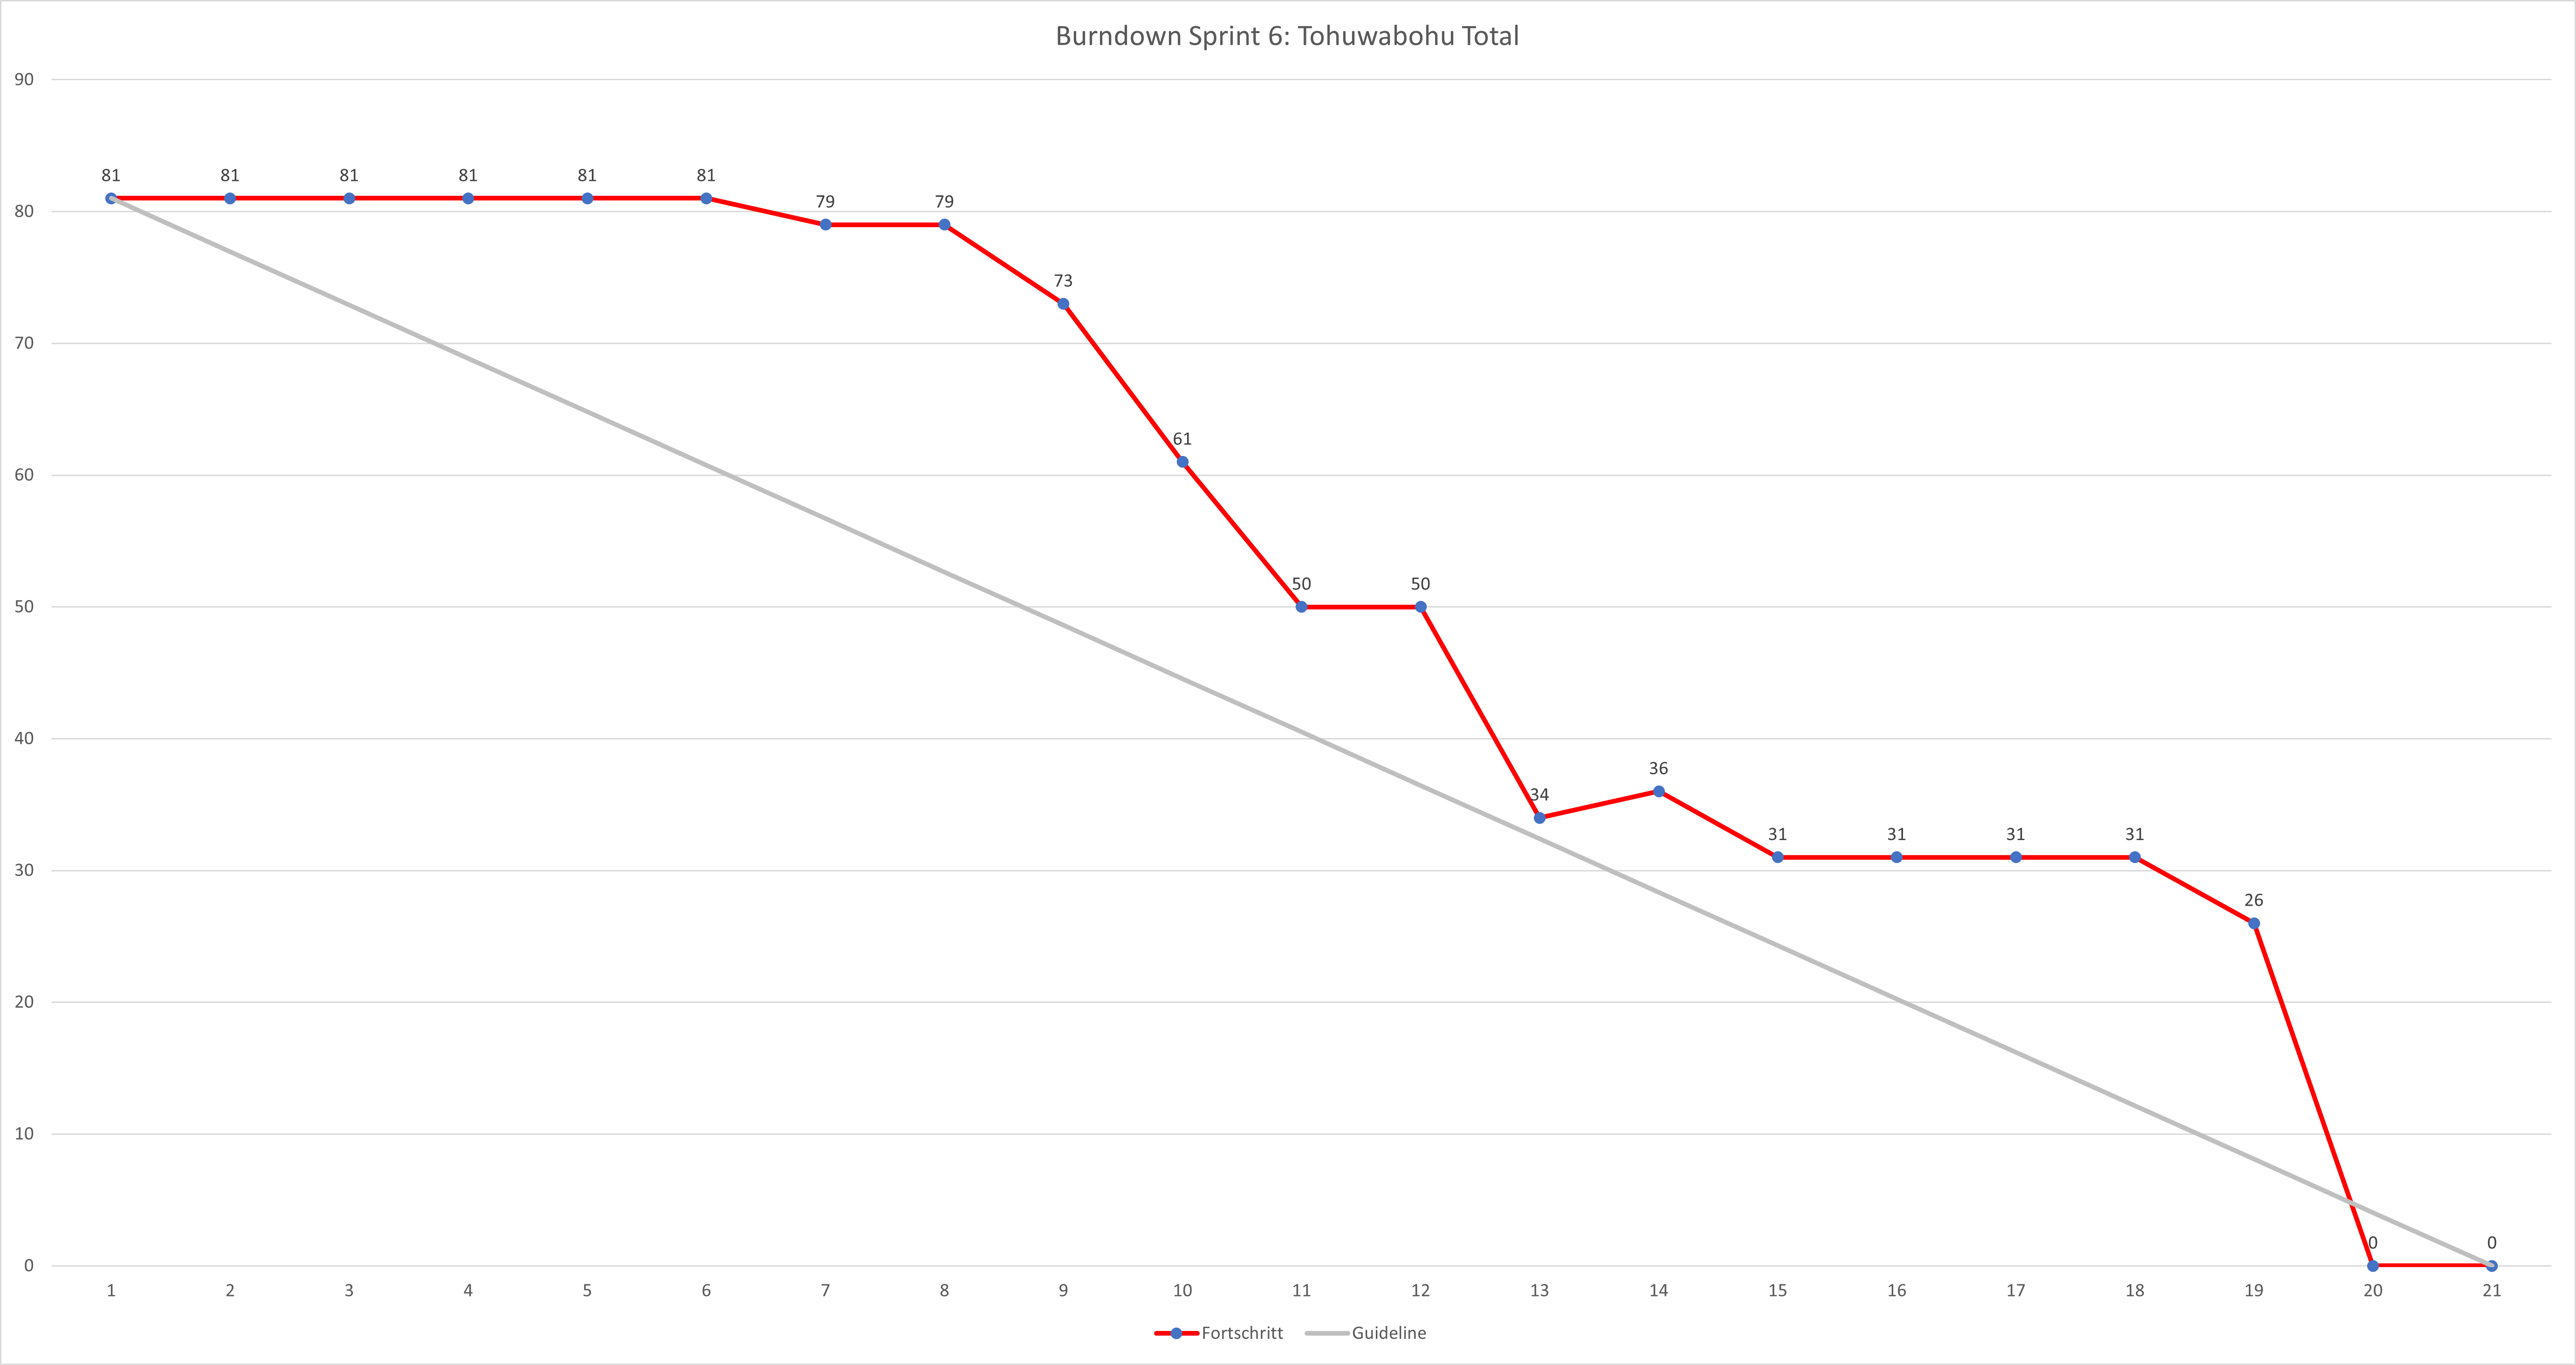
\includegraphics[width=\textwidth, height=5cm]{../img/sprint_06/Burndown-Sprint6.png}
    \caption{Burndown-Diagramm Sprint 6}
    \label{fig: Burndown-Sprint6}
\end{figure}
\noindent
Dieser Sprint war bisher der größte Sprint im Verlauf des Software-Projektes und betrug einen Gesamtaufwand von 83 Story Points. Aus dem Burndown-Diagramm wird ersichtlich, dass im frühem Verlauf des Sprints die Arbeitsaktivität eher gering war, wobei jedoch im mittleren Zeitraum die Aktivität deutlich gestiegen ist, aufgrund dessen, dass viele Vorgänge abgeschlossen wurden. Einige Gruppenmitlgieder hatten im mittleren Verlauf des Sprints bereits all ihre Vorgänge fertiggestellt, weshalb folgende Tasks zusätzlich dazugezogen wurden: \textit{SWP2020A-214: ANmi als Besitzer einer Lobby die anderen Lobbymitglieder rauswerfen können (1 Story Point)}, \textit{SWP2020A-215: StartSession-Button erscheint nach dem Handeln mit der Bank (1 Story Point)}, 
\textit{SWP2020A-213: X.setMessageContext(Y.getMessageContext()); durch X.initWithMessage(Y) ersetzen (1 Story Point).} Folglich wurde unser Sprintaufwand von 83 Story Points auf 86 Story Points erhöht und schlussendlich alle Vorgänge erfolgreich am 09. März 2021 abgeschlossen. 

\subsection{Sprintprobleme bzw. Hindernisse}
Zum Anfang des Sprints am 18. Februar 2021 bis hin zum 23. Februar 2021 hatte das Team keinerlei Fortschritt aufzuweisen anhand von abgeschlossenen Tasks. Das lag zum einen an einem Problem mit der Einbettung der in dem Sprint groß angelegten Dokumentation der vorherigen Sprints in Form von dem Sprinttagebuch. Hier wurden die einzelnen Sprintberichte nicht richtig in Bitbucket eingebunden und somit erfolgte der richtige Burndown dieser eigentlich früh im Sprint abgeschlossenen Tasks erst später. Zusätzlich dazu herrschte noch Klausurstress bei den meisten Teammitgliedern, weswegen sich der Erfolg in diesem Sprint zuerst in Grenzen hielt.


\newpage
\section{Erkenntnis aus der Retrospektive}
Folgende Erkenntnisse ergaben sich aus der Retrospektive:\\

\underline{Start:}
\begin{itemize}
    \item Wer mehr als 48 Stunden für eine Review braucht, kommt ans Burndown
    \item Wer zeitlich die Review nicht schafft, soll Bescheid geben, damit alternative Reviewer gefunden werden können
    \item Sub-Tasks beim Schätzen weniger extrem schätzen
    \item Button XY erstellen ist 0 Punkte
    \\
\end{itemize}

\underline{Stop:}
\begin{itemize}
    \item Früh anfangen zu arbeiten
    \item Nicht von der Länge eines Sprints zu Prokrastination verlocken lassen
    \item Jeder muss nach einer Woche etwas vorweisen (mind. Entwürfe / Konzepte)
    \item Bei Umfangsänderungswünschen Scrum-Master ansprechen
    \\
\end{itemize}

\underline{Weiter so:}
\begin{itemize}
    \item Auf Discord ansprechbar sein (max. 2 Tage für Antworten)
    \item Pair-Programming
\end{itemize}

\newpage
\section{Sonstige Anmerkungen}
Aus einem Versuch heraus am 03. März 2021, die Story Points der User Story \textit{SWP2020A-170: Spielfeldspeicherung überarbeiten (8 Story Points, nachgeschätzt auf 10 Story Points)}
anzupassen, wurde das Burndown-Diagramm für den Sprint 6 in Jira zerstört. Vermutlich aus dem Grund des Überschreiten eines Integer Wertebereichs zeigt das
Burndown-Diagramm aus Jira für diesen Sprint eine nicht repräsentative Grafik an, weshalb ein Excel-Diagramm zur korrekten Darstellung des Burndown-Diagramms eingebunden wurde.
\begin{figure}[h]
    \centering
    \includegraphics[width=\textwidth, height=5cm]{../img/sprint_06/Burndown-Sprint 6_zerstört.png}
    \caption{Burndown-Diagramm Sprint 6 laut Jira}
    \label{fig: Burndown-Sprint6_zerstört}
\end{figure}

\section{Fazit}
Generell lässt sich sagen, dass alles, was in diesem Sprint angestrebt wurde zu erreichen, auch erzielt wurde. Die anfängliche Arbeitsmoral, die einen geringen Erfolg mit sich zog schlug spätestens zur Mitte des Sprints um, sodass dieser Sprint mit zu den erfolgreichsten zählt, die das Team bisher zu verzeichnen hat. Mit 86 abgeschlossenen Story Points ist dieser Sprint auch der bis jetzt Umfangreichste.

\end{document}
